\documentclass[aspectratio=169,11pt]{beamer}
\usepackage[T1]{fontenc}
\usepackage{amsmath,amssymb}
\usepackage{tikz}
\usepackage{array}
\usepackage{booktabs}
\usepackage{ragged2e}
\usetikzlibrary{arrows.meta,positioning,calc}
\setbeamertemplate{navigation symbols}{}
\setbeamertemplate{footline}{}
\setbeamertemplate{headline}{}
\setbeamercolor{background canvas}{bg=white}
\setbeamercolor{normal text}{fg=black,bg=white}
\setbeamerfont{normal text}{size=\normalsize}
\setlength{\parindent}{0pt}

\definecolor{JPGray}{HTML}{777777}
\definecolor{JPLight}{HTML}{D7D7D7}
\definecolor{JPPaper}{HTML}{F5F5F5}
\definecolor{JPVeryLight}{HTML}{EFEFEF}

\newcommand{\jpheader}[3]{%
\begin{tikzpicture}[remember picture,overlay]
  \node[draw=black,rounded corners=2.5pt,minimum width=0.63cm,minimum height=0.50cm,line width=0.9pt,font=\bfseries\large] (n) at ([xshift=0.62cm,yshift=-0.47cm]current page.north west) {#1};
  \node[anchor=west,font=\bfseries\fontsize{13.0}{14.0}\selectfont] at ([xshift=0.25cm]n.east) {#2};
  \draw[JPLight,line width=0.7pt] ([xshift=0.42cm,yshift=-0.80cm]current page.north west) -- ([xshift=-0.42cm,yshift=-0.80cm]current page.north east);
  \node[anchor=north west,text width=14.2cm,align=left,font=\fontsize{10.7}{12.2}\selectfont] at ([xshift=0.42cm,yshift=-0.89cm]current page.north west) {#3};
\end{tikzpicture}
\vspace*{1.20cm}
}

\newcommand{\card}[3]{%
\begin{tikzpicture}
  \node[draw=black,rounded corners=3pt,line width=0.8pt,fill=white,inner xsep=7pt,inner ysep=6pt,text width=#1,align=left] {\textbf{#2}\\[2pt]#3};
\end{tikzpicture}%
}

\newcommand{\formulabox}[2][7.8cm]{%
\begin{tikzpicture}
\node[draw=black,rounded corners=3pt,line width=0.85pt,fill=JPPaper,inner xsep=7pt,inner ysep=6pt,text width=#1,align=center] {\Large $#2$};
\end{tikzpicture}%
}

\newcommand{\xtgraph}[1]{%
\begin{tikzpicture}[x=0.79cm,y=0.39cm,>=Latex]
  \foreach \xx in {1,...,7} {\draw[JPLight,line width=0.35pt] (\xx,0)--(\xx,10);}
  \foreach \yy in {2,4,6,8,10} {\draw[JPLight,line width=0.35pt] (0,\yy)--(7,\yy);}
  \draw[line width=0.95pt] (0,0)--(7.35,0);
  \draw[line width=0.95pt] (0,0)--(0,10.45);
  \foreach \xx in {0,...,7} {\draw[line width=0.65pt] (\xx,-0.18)--(\xx,0.18); \node[font=\scriptsize,below=2pt] at (\xx,0) {\xx};}
  \foreach \yy in {0,2,4,6,8,10} {\draw[line width=0.65pt] (-0.12,\yy)--(0.12,\yy); \node[font=\scriptsize,left=2pt] at (0,\yy) {\yy};}
  \node[font=\small,anchor=west] at (7.35,0) {$t$ (s)};
  \node[font=\small,anchor=south west] at (-0.25,10.45) {$x$ (m)};
  \draw[JPGray,dashed,line width=0.65pt] (3,0)--(3,10);
  \draw[JPGray,dashed,line width=0.65pt] (5,0)--(5,10);
  \draw[line width=1.4pt] (0,2)--(3,8);
  \draw[line width=1.4pt] (3,8)--(5,8);
  \draw[line width=1.4pt] (5,8)--(7,4);
  \ifnum#1=1 \draw[line width=3.0pt] (0,2)--(3,8);\fi
  \ifnum#1=2 \draw[line width=3.0pt] (3,8)--(5,8);\fi
  \ifnum#1=3 \draw[line width=3.0pt] (5,8)--(7,4);\fi
  \fill (0,2) circle (2.1pt); \fill (3,8) circle (2.1pt); \fill (5,8) circle (2.1pt); \fill (7,4) circle (2.1pt);
\end{tikzpicture}%
}

\newcommand{\vtgraph}[1]{%
\begin{tikzpicture}[x=0.79cm,y=0.68cm,>=Latex]
  \foreach \xx in {1,...,7} {\draw[JPLight,line width=0.35pt] (\xx,-3)--(\xx,3);}
  \foreach \yy in {-3,-2,-1,1,2,3} {\draw[JPLight,line width=0.35pt] (0,\yy)--(7,\yy);}
  \draw[line width=0.95pt] (0,0)--(7.35,0);
  \draw[line width=0.95pt] (0,-3.2)--(0,3.35);
  \foreach \xx in {0,...,7} {\draw[line width=0.65pt] (\xx,-0.09)--(\xx,0.09); \node[font=\scriptsize,below=2pt] at (\xx,0) {\xx};}
  \foreach \yy in {-3,-2,-1,0,1,2,3} {\draw[line width=0.65pt] (-0.10,\yy)--(0.10,\yy); \node[font=\scriptsize,left=2pt] at (0,\yy) {\yy};}
  \node[font=\small,anchor=west] at (7.35,0) {$t$ (s)};
  \node[font=\small,anchor=south west] at (-0.30,3.35) {$v$ (m/s)};
  \draw[JPGray,dashed,line width=0.65pt] (3,-3)--(3,3);
  \draw[JPGray,dashed,line width=0.65pt] (5,-3)--(5,3);
  \ifnum#1>0 \draw[line width=2.7pt] (0,2)--(3,2);\fi
  \ifnum#1>1 \draw[line width=2.7pt] (3,0)--(5,0);\fi
  \ifnum#1>2 \draw[line width=2.7pt] (5,-2)--(7,-2);\fi
\end{tikzpicture}%
}

\begin{document}

\begin{frame}[plain]
\begin{tikzpicture}[remember picture,overlay]
  \draw[JPLight,line width=0.8pt] ([xshift=2.1cm,yshift=-3.72cm]current page.north west) -- ([xshift=-2.1cm,yshift=-3.72cm]current page.north east);
\end{tikzpicture}
\vfill
\centering
{\large\bfseries PHYSICS 9 $\vert$ KINEMATICS}\par\vspace{0.35cm}
{\fontsize{30}{32}\selectfont\bfseries FROM POSITION GRAPH TO VELOCITY GRAPH}\par\vspace{0.45cm}
{\Large Use the exact Class 4-1 motion to construct the matching velocity-time graph}\par\vspace{0.60cm}
{\large\bfseries Slope on $x$-$t$ becomes height on $v$-$t$.}\par
\vfill
{\small Class 4-2 companion document}\par\vspace{0.25cm}
\end{frame}

\begin{frame}[plain]
\jpheader{01}{START FROM THE SAME POSITION-TIME GRAPH}{Do not invent new motion data. Reuse the exact four events from Class 4-1 and identify the three straight motion intervals.}
\begin{columns}[T,onlytextwidth]
\column{0.58\textwidth}
\centering
\xtgraph{0}
\column{0.39\textwidth}
\vspace{0.18cm}
\card{5.1cm}{EXACT MOTION DATA}{\small $(0\,\mathrm{s},2\,\mathrm{m})\rightarrow(3\,\mathrm{s},8\,\mathrm{m})$\\$\rightarrow(5\,\mathrm{s},8\,\mathrm{m})\rightarrow(7\,\mathrm{s},4\,\mathrm{m})$}
\vspace{0.30cm}
\card{5.1cm}{THREE INTERVALS}{\small 0 to 3 s: rising\\3 to 5 s: horizontal\\5 to 7 s: falling}
\vspace{0.28cm}
\formulabox[5.1cm]{v=\text{slope}=\dfrac{\Delta x}{\Delta t}}
\end{columns}
\end{frame}

\begin{frame}[plain]
\jpheader{02}{CALCULATE ONE SLOPE FOR EACH STRAIGHT SEGMENT}{Velocity is not read from graph height. It is the slope: change in position divided by change in time.}
\begin{columns}[T,onlytextwidth]
\column{0.55\textwidth}
\centering
\xtgraph{1}
\column{0.42\textwidth}
\vspace{0.25cm}
{\Large\bfseries INTERVAL 1: $0\le t<3\,\mathrm{s}$}\par\vspace{0.42cm}
{\Large $\Delta x = 8-2 = +6\,\mathrm{m}$}\par\vspace{0.27cm}
{\Large $\Delta t = 3-0 = 3\,\mathrm{s}$}\par\vspace{0.37cm}
\formulabox[5.4cm]{v=\dfrac{+6}{3}=+2\,\mathrm{m/s}}
\vspace{0.38cm}
\card{5.4cm}{VELOCITY LEVEL: +2 m/s}{\small This becomes one horizontal segment on the velocity-time graph over 0 to 3 s.}
\end{columns}
\end{frame}

\begin{frame}[plain]
\jpheader{02}{CALCULATE ONE SLOPE FOR EACH STRAIGHT SEGMENT}{The horizontal segment has zero rise, therefore zero velocity even though the position is $8\,\mathrm{m}$.}
\begin{columns}[T,onlytextwidth]
\column{0.55\textwidth}
\centering
\xtgraph{2}
\column{0.42\textwidth}
\vspace{0.25cm}
{\Large\bfseries INTERVAL 2: $3\le t<5\,\mathrm{s}$}\par\vspace{0.42cm}
{\Large $\Delta x = 8-8 = 0\,\mathrm{m}$}\par\vspace{0.27cm}
{\Large $\Delta t = 5-3 = 2\,\mathrm{s}$}\par\vspace{0.37cm}
\formulabox[5.4cm]{v=\dfrac{0}{2}=0\,\mathrm{m/s}}
\vspace{0.38cm}
\card{5.4cm}{VELOCITY LEVEL: 0 m/s}{\small Position is constant during this interval: the object is at rest.}
\end{columns}
\end{frame}

\begin{frame}[plain]
\jpheader{02}{CALCULATE ONE SLOPE FOR EACH STRAIGHT SEGMENT}{A falling position-time segment has negative slope, so the velocity is negative.}
\begin{columns}[T,onlytextwidth]
\column{0.55\textwidth}
\centering
\xtgraph{3}
\column{0.42\textwidth}
\vspace{0.25cm}
{\Large\bfseries INTERVAL 3: $5\le t\le7\,\mathrm{s}$}\par\vspace{0.42cm}
{\Large $\Delta x = 4-8 = -4\,\mathrm{m}$}\par\vspace{0.27cm}
{\Large $\Delta t = 7-5 = 2\,\mathrm{s}$}\par\vspace{0.37cm}
\formulabox[5.4cm]{v=\dfrac{-4}{2}=-2\,\mathrm{m/s}}
\vspace{0.38cm}
\card{5.4cm}{VELOCITY LEVEL: -2 m/s}{\small This becomes one horizontal segment below the time axis over 5 to 7 s.}
\end{columns}
\end{frame}

\begin{frame}[plain]
\jpheader{03}{YOUR TURN: CONSTRUCT THE VELOCITY-TIME GRAPH}{Before the answer appears, use the three velocities you calculated and place each one over its correct time interval.}
\vspace{0.55cm}
\begin{columns}[T,onlytextwidth]
\column{0.58\textwidth}
\centering
\scalebox{0.72}{\vtgraph{0}}
\column{0.38\textwidth}
\vspace{0.75cm}
\card{4.8cm}{STUDENT TASK}{\small Draw one horizontal segment for each interval. Use the correct sign and keep the same time boundaries at $t=3$ s and $t=5$ s.}
\end{columns}
\vspace{0.16cm}
\begin{columns}[T,onlytextwidth]
\column{0.32\textwidth}\centering
\card{3.6cm}{INTERVAL 1}{\small 0 to 3 s\\$v=+2\,\mathrm{m/s}$}
\column{0.32\textwidth}\centering
\card{3.6cm}{INTERVAL 2}{\small 3 to 5 s\\$v=0\,\mathrm{m/s}$}
\column{0.32\textwidth}\centering
\card{3.6cm}{INTERVAL 3}{\small 5 to 7 s\\$v=-2\,\mathrm{m/s}$}
\end{columns}
\end{frame}

\begin{frame}[plain]
\jpheader{04}{BUILD THE VELOCITY GRAPH ONE INTERVAL AT A TIME}{Each constant slope on the position graph becomes a constant height on the velocity graph over the same time interval.}
\begin{columns}[T,onlytextwidth]
\column{0.57\textwidth}
\centering
\vtgraph{3}
\vspace{0.18cm}
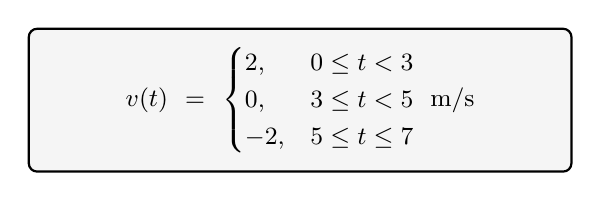
\begin{tikzpicture}
\node[draw=black,rounded corners=3pt,line width=0.8pt,fill=JPPaper,inner xsep=7pt,inner ysep=6pt,text width=6.4cm,align=center] {
\small $\displaystyle v(t)=\begin{cases}
2,&0\le t<3\\
0,&3\le t<5\\
-2,&5\le t\le 7
\end{cases}\ \mathrm{m/s}$};
\end{tikzpicture}
\column{0.40\textwidth}
\vspace{0.06cm}
\card{5.0cm}{STEP 1}{\small 0 to 3 s: plot $v=+2\,\mathrm{m/s}$}
\vspace{0.09cm}
\card{5.0cm}{STEP 2}{\small 3 to 5 s: plot $v=0\,\mathrm{m/s}$}
\vspace{0.09cm}
\card{5.0cm}{STEP 3}{\small 5 to 7 s: plot $v=-2\,\mathrm{m/s}$}
\vspace{0.15cm}
\card{5.0cm}{AT $t=3$ s AND $t=5$ s}{\small Velocity changes instantly at the idealized boundaries. Do not connect the levels vertically.}
\end{columns}
\end{frame}

\begin{frame}[plain]
\jpheader{05}{COMPARE THE TWO REPRESENTATIONS}{Look vertically at the same time interval: slope on $x$-$t$ and height on $v$-$t$ must describe the same motion.}
\begin{columns}[T,onlytextwidth]
\column{0.49\textwidth}
\centering
{\Large\bfseries POSITION-TIME}\par\vspace{0.10cm}
\resizebox{0.93\linewidth}{!}{\xtgraph{0}}
\column{0.49\textwidth}
\centering
{\Large\bfseries VELOCITY-TIME}\par\vspace{0.10cm}
\resizebox{0.93\linewidth}{!}{\vtgraph{3}}
\end{columns}
\vspace{0.12cm}
\begin{columns}[T,onlytextwidth]
\column{0.32\textwidth}\centering
\card{3.8cm}{RISING $x$-$t$}{\small same time interval\\$v=+2\,\mathrm{m/s}$}
\column{0.32\textwidth}\centering
\card{3.8cm}{HORIZONTAL $x$-$t$}{\small same time interval\\$v=0\,\mathrm{m/s}$}
\column{0.32\textwidth}\centering
\card{3.8cm}{FALLING $x$-$t$}{\small same time interval\\$v=-2\,\mathrm{m/s}$}
\end{columns}
\end{frame}

\begin{frame}[plain]
\jpheader{06}{CHECK THE PHYSICS, NOT ONLY THE DRAWING}{A correct velocity graph must reproduce direction, rest, and the net displacement of the original motion.}
\begin{columns}[T,onlytextwidth]
\column{0.32\textwidth}\centering
\card{3.9cm}{0-3 s $\vert$ MOVE RIGHT}{\small $x$ increases by $6\,\mathrm{m}$\\$v=+2\,\mathrm{m/s}$}
\column{0.32\textwidth}\centering
\card{3.9cm}{3-5 s $\vert$ WAIT}{\small $x$ stays at $8\,\mathrm{m}$\\$v=0\,\mathrm{m/s}$}
\column{0.32\textwidth}\centering
\card{3.9cm}{5-7 s $\vert$ RETURN LEFT}{\small $x$ decreases by $4\,\mathrm{m}$\\$v=-2\,\mathrm{m/s}$}
\end{columns}
\vspace{0.48cm}
\centering
{\Large $\Delta x=(+2)(3)+(0)(2)+(-2)(2)$}\par\vspace{0.22cm}
{\Large $\Delta x=6+0-4=+2\,\mathrm{m}$}\par\vspace{0.27cm}
\formulabox[7.0cm]{x_f=x_i+\Delta x=2+2=4\,\mathrm{m}}\par
\vspace{0.34cm}
{\small The signed area under the $v$-$t$ graph reproduces the final position of the original $x$-$t$ graph.}
\end{frame}

\begin{frame}[plain]
\jpheader{07}{THE FIVE-STEP $x$-$t$ TO $v$-$t$ METHOD}{Use this exact sequence whenever a piecewise position-time graph is made of straight segments.}
\vspace{0.30cm}
\begin{columns}[T,onlytextwidth]
\column{0.19\textwidth}\centering
\card{2.5cm}{1 $\vert$ SPLIT}{\small Mark every straight time interval.}
\column{0.19\textwidth}\centering
\card{2.5cm}{2 $\vert$ SLOPE}{\small Compute $\Delta x/\Delta t$.}
\column{0.19\textwidth}\centering
\card{2.5cm}{3 $\vert$ SIGN}{\small Rising $+$, flat $0$, falling $-$.}
\column{0.19\textwidth}\centering
\card{2.5cm}{4 $\vert$ HEIGHT}{\small Plot that $v$ level on the same interval.}
\column{0.19\textwidth}\centering
\card{2.5cm}{5 $\vert$ CHECK}{\small Area under $v$-$t$ must match $\Delta x$.}
\end{columns}
\vspace{0.60cm}
\centering
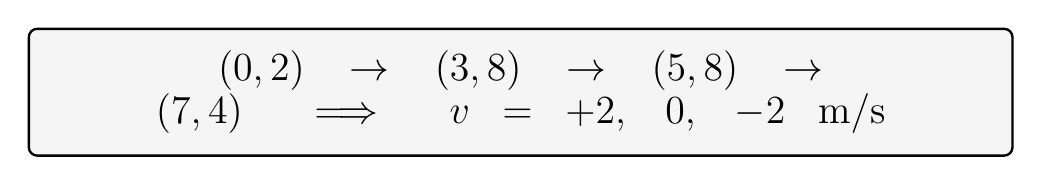
\begin{tikzpicture}
\node[draw=black,rounded corners=3pt,line width=0.85pt,fill=JPPaper,inner xsep=7pt,inner ysep=8pt,text width=12.0cm,align=center] {\Large $(0,2)\rightarrow(3,8)\rightarrow(5,8)\rightarrow(7,4)\quad\Longrightarrow\quad v=+2,\;0,\;-2\;\mathrm{m/s}$};
\end{tikzpicture}
\vspace{0.48cm}
{\LARGE\bfseries SLOPE ON $x$-$t$ = HEIGHT ON $v$-$t$}\par\vspace{0.40cm}
{\large Construct. Calculate. Match the interval. Verify the motion.}
\end{frame}

\end{document}
